\section{Comparisons}
\subsection{QNNs vs NNs}\label{sec:qnn-vs-nn}

In order to compare the performance of the QNN and the NN, architectures suited for binary classification with exactly 8 parameters are used.
The QNN structure is shown in \cref{fig:qnn_vs_nn_models}.
The data used is Fisher's iris dataset, perhaps the most used dataset for studying classification in statistics, containing samples of three different species of iris flowers.
For each species, there are 50 samples, each with four features: sepal length, sepal width, petal length, and petal width.
Like in \cite{abbas2021}, only the two first species are considered, which happen to be linearly separable in the feature space.

The four-dimensional input data is first scaled to have zero mean and unit variance.
Then, it is encoded into a quantum state a second order angle encoding with $Z$ rotations, discussed in \cref{sec:second_order_angle_encoding}, with two repetitions.
In the Qiskit framework, this is implemented in the \texttt{ZZFeatureMap} class.
This entangles the qubits and embeds them in higher dimensional space.

Next, the state is evolved by the parametrised circuit.
It consists of initial parametrised Y-rotations, then full entanglement using controlled not-gates, and lastly final parametrised Y-rotations.
The different rotation direction ensures the gates do not commute.
There are in total 8 parameters.
This is implemented in Qiskit as the \texttt{RealAmplitudes} ansatz.

Finally, all four qubits are measured and the parity of the four bit output is interpreted as the prediction of the class label.  \Cref{fig:qnn_vs_nn_models} shows the structure of the QNN and how the parameters are used.

Both exact simulations and noisy simulations were performed, with the latter using noise modelled after the 27-qubit IBM Montreal architecture, the actual hardware used in the original paper.

\begin{figure}
    \centering
    \begin{quantikz}
        \lstick{$\ket{0}$} &
        \gate[wires=4, disable auto height]{{\rotatebox{90}{\texttt{ZZFeatureMap}$(\bm{x})$}}} &
        \gate{R_Y(\theta_1)}
        \gategroup[
            wires=4,
            steps=8,
            style={dashed, rounded corners, inner sep=2pt},
            label style={label position=below, anchor=north, yshift=-0.2cm},
        ]{
            \texttt{RealAmplitudes}$(\bm{\theta})$
        }
        &
        \ctrl{1} &
        \ctrl{2} &
        \ctrl{3} &
        \qw &
        \qw &
        \qw &
        \gate{R_Y(\theta_5)} &
        \meter{}
        \\
        \lstick{$\ket{0}$} &
        \qw &
        \gate{R_Y (\theta_2)} &
        \targ{} &
        \qw &
        \qw &
        \ctrl{1} &
        \ctrl{2} &
        \qw &
        \gate{R_Y(\theta_6)} &
        \meter{}
        \\
        \lstick{$\ket{0}$} &
        \qw &
        \gate{R_Y (\theta_3)} &
        \qw &
        \targ{} &
        \qw &
        \targ{} &
        \qw &
        \ctrl{1} &
        \gate{R_Y(\theta_7)} &
        \meter{}
        \\
        \lstick{$\ket{0}$} &
        \qw &
        \gate{R_Y (\theta_4)} &
        \qw &
        \qw &
        \targ{}&
        \qw &
        \targ{}&
        \targ{}&
        \gate{R_Y(\theta_8)} &
        \meter{}
    \end{quantikz}
    \caption{
        Structure of the QNN used for classification of the iris dataset.
        The first block maps the input data $\bm{x}$ to the quantum state $\ket{\psi(\bm{x})}$ using a second order $Z$ rotation feature map.
        The second block is the variational circuit, parametrised by $\bm{\theta}$, a vector with eight components.
        Finally, all qubits are measured, where the parity is interpreted as the prediction.
    }
    \label{fig:qnn_vs_nn_models}
\end{figure}

The classical neural network was a standard dense feed-forward model.
To make in comparable to the QNN, it used a 4-1-1-1-2 layered structure without biases, giving a total of 8 parameters.
The activation functions were leaky ReLUs,
\begin{equation}
    \text{LeakyReLU}(x) = \begin{cases}
        x     & x \geq 0 \\
        0.01x & x < 0
    \end{cases},
\end{equation}
and the output layer used a softmax activation function.

Both models were implemented using PyTorch, with code partly taken from the original paper\footnote{Available at \url{https://github.com/amyami187/effective_dimension}.}.
The QNN was adapted to use Qiskit's PyTorch interface.
Consequently, the models could be trained in the exact same manner, using the Adam optimiser with a learning rate of 0.1 and cross-entropy loss.
The classical and noiseless models were trained for 100 epochs, while the noisy model was only trained for 10, as simulating the noise severely impacted training time.

For validation, 10-fold cross-validation was used.
That is, the dataset was split into 10 equal parts (folds).
Each fold us used as the validation set once, their accuracies being recorded during the training with the other nine folds.
The mean accuracy over the 10 folds was used for the final performance metric, shown in \cref{fig:iris_training}.

\begin{figure}
    \centering
    \begin{tikzpicture}
        \begin{axis}[
                width=0.8\textwidth,
                height=0.5\textwidth,
                xlabel={Iteration},
                ylabel={Mean out-of-fold accuracy},
                grid = major,
                legend pos=south east,
                legend cell align={left},
            ]
            \addplot[mark=none, color=red] table[x expr=\coordindex+1, y index=3, col sep=comma] {../code/iris/results/mean.csv};
            \addplot[mark=none, color=blue] table[x expr=\coordindex+1, y index=2, col sep=comma] {../code/iris/results/mean.csv};
            \addplot[mark=none, color=green] table[x expr=\coordindex+1, y index=1, col sep=comma] {../code/iris/results/mean.csv};
            \legend{
                Noisy QNN,
                Exact QNN,
                Classical NN
            }
        \end{axis}
    \end{tikzpicture}
    \caption{
        Mean accuracies during training for the iris dataset.
        Ten-fold cross-validation was used, with the mean out-of-fold accuracy being used as the final performance metric.
        All models have 8 parameters and are trained using the Adam optimiser with a learning rate of 0.1, using cross-entropy as the loss function.
        Due to the computational cost, the noisy (simulated IBM Montreal backend) QNN was only trained for ten epochs.
    }
    \label{fig:iris_training}
\end{figure}


As in the original paper, the QNN converges much quicker and more consistently, with an out-of-fold accuracy of 100\% for all ten folds.
The classical network, on the other hand, requires more iterations to converge and does not always do so.
In some cases, the model did not converge, only predicting one class, which is why the out-of-fold accuracy was not 100\% for all folds.
This is in line with the original paper, underlining the potential advantage of quantum neural networks.


\subsection{Quantum convolutional neural networks}
\label{sec:qcnn}
% Quantum convolutional neural networks work similarly to classical convolutional networks. Through iterated convolution and pooling layers where only spatially 'near' features affect each other in the first layers, the total amount of parameters is reduced relative to fully connected networks, and the CNN tends to learn more local features. This makes them well suited for image classification, where the significant features are often spatially correlated and global features such as the local of the subject in the image does not matter.

To implement and test a quantum CNN, Qiskit's online tutorials were closely followed \cite{qiskit_qcnn}.
Being limited to few qubits, images with resolution $2\times4$ were generated, containing either vertical or horizontal with some Gaussian noise.
\Cref{fig:qcnn_data} shows examples thereof.
The task of the QCNN was to classify the images as either vertical or horizontal lines.

\begin{figure}
    \centering
    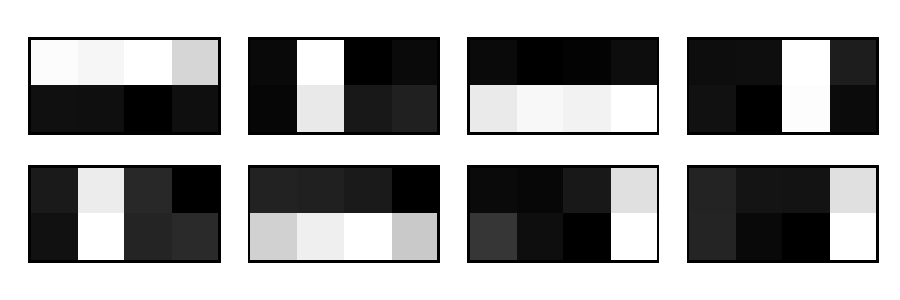
\includegraphics[width=\textwidth]{../code/qcnn/data.pdf}
    \caption{
        Data for the QCNN.
        With a total of 64 training images and 16 for testing, they form balanced dataset of $2\times4$ pixels, with either a vertical or horizontal line encoded as $1$ and $-1$.
        The images are generated with some Gaussian noise.
    }
    \label{fig:qcnn_data}
\end{figure}


First, data is encoded using two repetitions of $Z$ angle encoding, implemented in Qiskit as the \texttt{ZFeatureMap}.
Each of the eight pixels of the image is mapped to a qubit through two repetitions of the Hadamard gate and $Z$-rotations parametrised by the pixel value being applied, in circuit notation:

\begin{equation}
    \begin{quantikz}
        \lstick{$\ket{0}$} & \gate{H} & \gate{R_Z(x_1)} & \gate{H} & \gate{R_Z(x_1)}  \\
        \lstick{$\ket{0}$} & \gate{H} & \gate{R_Z(x_2)} & \gate{H} & \gate{R_Z(x_2)}  \\
        \lstick{\vdots} \\
        \lstick{$\ket{0}$} & \gate{H} & \gate{R_Z(x_n)} & \gate{H} & \gate{R_Z(x_n)}  \\
    \end{quantikz}
\end{equation}



The convolution layers act with pairwise parametrised rotations of neighbouring qubits, also wrapping around, entangling the first and last qubits through various CNOT gates and both parametrised and fixed $Z$ and $Y$ rotations.
Effectively, each consecutive pair of qubits were entangled by
\begin{equation}
    \begin{quantikz}
        &
        \qw
        &
        \targ{}
        &
        \gate{R_Z(\theta_{0})}
        &
        \ctrl{1}
        &
        \qw
        &
        \targ{}
        &
        \gate{R_Z(\pi/2)}
        &
        \qw
        \\
        &
        \gate{R_Z(-\pi/2)}
        &
        \ctrl{-1}
        &
        \gate{R_Y(\theta_{1})}
        &
        \targ{}
        &
        \gate{R_Y(\theta_{3})}
        &
        \ctrl{-1}
        &
        \qw
        &
        \qw
    \end{quantikz}
\end{equation}
giving $3n$ parameters for each convolution layer of $n$ qubits.


Thereafter, pooling layers halve the active qubit counts by parametrised rotations and CNOT gates.
This is done by acting on the first and fifth, second and sixth et cetera with the following circuit:
\begin{equation}
    \begin{quantikz}
        &
        \qw
        &
        \targ{}
        &
        \gate{R_Z(\theta_{0})}
        &
        \ctrl{1}
        &
        \qw
        &
        \qw
        \\
        &
        \gate{R_Z(-\pi/2)}
        &
        \ctrl{-1}
        &
        \gate{R_Y(\theta_{1})}
        &
        \targ{}
        &
        \gate{R_Y(\theta_{3})}
        &
        \qw
    \end{quantikz}
\end{equation}
giving $3n/2$ parameters for each pooling layer of $n$ qubits.

For the final layer, the sole remaining qubit is measured, and the result is interpreted as the prediction.
In total, the circuit appears as
\begin{center}
    \begin{quantikz}
        \lstick[wires=8]{$\ket{0}^{\otimes 8}$} &
        \gate[wires=8, disable auto height]{{\rotatebox{90}{\texttt{ZFeatureMap}$(\bm{x})$}}} &
        \gate[wires=8, disable auto height]{{\rotatebox{90}{\text{Convolution}}}} &
        \gate[wires=8, disable auto height]{{\rotatebox{90}{\text{Pooling}}}} & \qw{}& \qw{}& \qw{}& \qw{} & \qw{}
        \\
        & \qw{}& \qw{}& \qw{}& \qw{}& \qw{}& \qw{}& \qw{}& \qw{}\\
        & \qw{}& \qw{}& \qw{}& \qw{}& \qw{}& \qw{}& \qw{}& \qw{}\\
        & \qw{}& \qw{}& \qw{}& \qw{}& \qw{}& \qw{}& \qw{}& \qw{}\\
        & & & &
        \gate[wires=4, disable auto height]{{\rotatebox{90}{\text{Convolution}}}} &
        \gate[wires=4, disable auto height]{{\rotatebox{90}{\text{Pooling}}}} & \qw{} & \qw{} & \qw{}
        \\
        & \qw{}& \qw{}& \qw{}& \qw{}& \qw{}& \qw{}& \qw{}& \qw{}\\
        & & & & & &
        \gate[wires=2, disable auto height]{{\rotatebox{90}{\text{Conv.}}}} &
        \gate[wires=2, disable auto height]{{\rotatebox{90}{\text{Pooling}}}} & \qw{}

        \\
        & & & & & & & & \meter{} \\
    \end{quantikz}
\end{center}
with a total of 63 parameters.


As in Qiskit's guide, training was done using the COBYLA optimiser\footnote{Constrained Optimisation BY Linear Approximation.} which does not use gradients.
Why this optimiser was chosen is not clear, but testing shows that simulations using gradient based methods such as Adam or simple gradient descent is significantly slower.
The accuracies and loss (mean square error) during training is shown in \cref{fig:qcnn_training}.
Like in \cref{sec:qnn-vs-nn}, noise is modelled after the IBM Montreal hardware.
The networks were trained for 1000 epochs, and while neither reached full accuracy, the losses shrunk, indicating at least increased certainty in the predictions.
Interestingly, the noisy simulation appears to yield better predictions, despite suffering from higher losses during training.
It seems that the noiseless QCNN is overfitting to the training data, while the noisy QCNN generalises better.


\begin{figure}
    \centering
    \begin{subfigure}{0.49\textwidth}
        \centering
        \begin{tikzpicture}
            \begin{axis}[
                    width=\textwidth,
                    height=\textwidth,
                    xlabel={Iteration},
                    ylabel={Loss (MSE)},
                    % legend pos=north west,
                    % legend style={at={(0.5,1.03)},anchor=north},
                    grid=major,
                    xtick distance=200,
                ]
                \addplot[mark=none, color=red] table[x=iteration, y=loss, col sep=comma] {../code/qcnn/noisy.csv};
                \addplot[mark=none, color=blue] table[x=iteration, y=loss, col sep=comma] {../code/qcnn/exact.csv};
                \legend{
                    Noisy QCNN,
                    Exact QCNN,
                }
            \end{axis}
        \end{tikzpicture}
        \caption{}
        \label{fig:qcnn_loss}
    \end{subfigure}
    \begin{subfigure}{0.49\textwidth}
        \centering
        \begin{tikzpicture}
            \begin{axis}[
                    width=\textwidth,
                    height=\textwidth,
                    xlabel={Iteration},
                    ylabel={Accuracy},
                    % legend pos=north west,
                    % legend style={at={(0.5,1.03)},anchor=north},
                    grid=major,
                    legend pos=south east,
                    xtick distance=200,
                ]
                % \addplot[mark=none, color=red] table[x=iteration, y=training_acc, col sep=comma] {../code/qcnn/noisy.csv};
                % \addplot[mark=none, color=red, dashed] table[x=iteration, y=test_acc, col sep=comma] {../code/qcnn/noisy.csv};
                % \addplot[mark=none, color=blue] table[x=iteration, y=training_acc, col sep=comma] {../code/qcnn/exact.csv};
                % \addplot[mark=none, color=blue, dashed] table[x=iteration, y=test_acc, col sep=comma] {../code/qcnn/exact.csv};
                \addplot[mark=none, color=red] table[x=iteration, y=train_mean_noisy, col sep=comma] {../code/qcnn/mean_accs.csv};
                \addplot[mark=none, color=red, dashed] table[x=iteration, y=test_mean_noisy, col sep=comma] {../code/qcnn/mean_accs.csv};
                \addplot[mark=none, color=blue] table[x=iteration, y=train_mean_exact, col sep=comma] {../code/qcnn/mean_accs.csv};
                \addplot[mark=none, color=blue, dashed] table[x=iteration, y=test_mean_exact, col sep=comma] {../code/qcnn/mean_accs.csv};
                \legend{
                    Noisy training,
                    Noisy test,
                    Exact training,
                    Exact test,
                }
            \end{axis}
        \end{tikzpicture}
        \caption{}
        \label{fig:qcnn_acc}
    \end{subfigure}
    \caption{
        Training of the basic QCNN.
        The red curves are for the noisy model (modelled after IBM's Montreal hardware), while the blue curves are for the exact model.
        The dashed curves are for the test set.
        (a) loss (mean square error) during training.
        (b) accuracy on the training and test sets (running mean with a 100 iteration window).
    }
    \label{fig:qcnn_training}
\end{figure}


\subsection{QCNN with intermediate measurements}
A more complex QCNN structure was described by \textcite{pesah2021}, where the pooling modules measure a qubit and use the result to control a unitary gate on its neighbour.
The use of mid-circuit measurements complicates the circuit and its implementation, but allows for a non-linear and potentially more powerful model.

Following the description in \cite{pesah2021}, a QCNN was implemented with structure as shown in \cref{fig:qcnnm}.
First, the data was encoded using angle encoding in the $X$ direction.
The convolutional layers consisted of pairwise $W$ gates, a mix of parametrised rotations and CNOTs, with total of 15 parameters per gate.
The pooling layers consisted of a measurement and a conditional single-qubit unitary gate.
Without any particular recommendation in the original paper, a simple $X$-gate was used.
Like in \cref{sec:qcnn}, the network used 8 qubits to handle the 8-dimensional data.
Three convolutional and pooling layers were used, reducing the data from 8 to 2 dimensions
Lastly, a final general two-qubit ansatz was used, and a single qubit was measured and interpreted as a prediction.
This was a simple parametrised entangler, similar to the \texttt{RealAmplitudes} in \cref{sec:qnn-vs-nn}, but with $X$ rotations.
In total, the network had 154 parameters.

\begin{figure}
    \centering
    \begin{quantikz}
        % \lstick[wires=4]{$\ket{\psi(\bm{x})}$}
        &
        \qw
        \gategroup[
            wires=4,
            steps=2,
            style={dashed, rounded corners, inner sep=2pt},
            label style={label position=below, anchor=north, yshift=-0.2cm},
        ]{Convolution}
        &
        \gate[wires=2]{W}
        &
        \qw
        &
        \meter{}
        \gategroup[
            wires=4,
            steps=2,
            style={dashed, rounded corners, inner sep=2pt},
            label style={label position=below, anchor=north, yshift=-0.2cm},
        ]{Pooling}
        &
        \cwbend{1}
        \\
        &
        \gate[wires=2]{W}
        &
        \qw
        &
        \qw
        &
        \qw
        &
        \gate{X}
        &
        \qw
        \\
        &
        \qw
        &
        \gate[wires=2]{W}
        &
        \qw
        &
        \qw
        &
        \gate{X}
        &
        \qw
        \\
        &
        \qw
        &
        \qw
        &
        \qw
        &
        \meter{}
        &
        \cwbend{-1}
    \end{quantikz}
    \caption{
        QCNN convolution and pooling layer structure with intermediate measurements.
        Some encoded data or already pooled data enter the convolution layer where parametrised gates $W$ entangle the qubits.
        The pooling modules measure a qubit and use the result to control a unitary gate on a neighbour (here the $X$ gate).
    }
    \label{fig:qcnnm}
\end{figure}

The QCNN was implemented using the PennyLane framework and trained with the Adam optimiser with a learning rate of 0.01.
With the PennyLane implementation, there were no problems using gradient based optimisation.
This prompted the reimplementation of the former QCNN, which was here also trained with the same Adam optimiser.
The results are shown in \cref{fig:qcnnm_training}.
The training loss was lower than for the QCNN in \cref{sec:qcnn}, despite the fewer iterations, showing expected advantages of using gradient based optimisation.
Furthermore, the new model with intermediate measurements achieves a perfect accuracy on both the training and test sets in only 10 iterations.
Looking at the loss curves, the model with intermediate measurements seems only to converge slightly faster than the model without intermediate measurements.
However, by extending the model without mid-circuit measurements to have a more comparable parameter count of 231, it overtakes the model with intermediate measurements in terms of training loss.

\begin{figure}
    \centering
    \begin{subfigure}{0.49\textwidth}
        \centering
        \begin{tikzpicture}
            \begin{axis}[
                    width=\textwidth,
                    height=\textwidth,
                    xlabel={Iteration},
                    ylabel={Loss (MSE)},
                    % legend pos=north west,
                    % legend style={at={(0.5,1.03)},anchor=north},
                    grid=major,
                    legend pos=north east,
                    ymode=log,
                ]
                \addplot[mark=none, color=blue] table[x=Iteration, y=Loss, col sep=comma] {../code/qcnn_pennylane/results_intermediate.csv};
                \addplot[mark=none, color=red] table[x=Iteration, y=Loss, col sep=comma] {../code/qcnn_pennylane/results_simple.csv};
                \addplot[mark=none, color=green] table[x=Iteration, y=Loss, col sep=comma] {../code/qcnn_pennylane/results_simple_ext.csv};
                \legend{
                    With intermediate,
                    Without,
                    Without extended
                }
            \end{axis}
        \end{tikzpicture}
        \caption{}
        \label{fig:qcnnm_loss}
    \end{subfigure}
    \begin{subfigure}{0.49\textwidth}
        \centering
        \begin{tikzpicture}
            \begin{axis}[
                    width=\textwidth,
                    height=\textwidth,
                    xlabel={Iteration},
                    ylabel={Accuracy},
                    % legend pos=north west,
                    % legend style={at={(0.5,1.03)},anchor=north},
                    grid=major,
                    legend pos=south east,
                    xmax=35,
                ]
                \addplot[mark=none, color=blue] table[x=Iteration, y=Accuracy, col sep=comma] {../code/qcnn_pennylane/results_intermediate.csv};
                \addplot[mark=none, color=blue, dashed] table[x=Iteration, y=Test accuracy, col sep=comma] {../code/qcnn_pennylane/results_intermediate.csv};
                \addplot[mark=none, color=red] table[x=Iteration, y=Accuracy, col sep=comma] {../code/qcnn_pennylane/results_simple.csv};
                \addplot[mark=none, color=red, dashed] table[x=Iteration, y=Test accuracy, col sep=comma] {../code/qcnn_pennylane/results_simple.csv};
                \addplot[mark=none, color=green] table[x=Iteration, y=Accuracy, col sep=comma] {../code/qcnn_pennylane/results_simple_ext.csv};
                \addplot[mark=none, color=green, dashed] table[x=Iteration, y=Test accuracy, col sep=comma] {../code/qcnn_pennylane/results_simple_ext.csv};
                \legend{
                    With intermediate,
                    , %With intermediate (test),
                    Without,
                    , %Without (test),
                    Without extended,
                    , %Without extended (test)
                }
            \end{axis}
        \end{tikzpicture}
        \caption{}
        \label{fig:qcnnm_acc}
    \end{subfigure}
    \caption{
        Training of QCNNs with and without intermediate measurements.
        With intermediate refers to the QCNN with intermediate measurements of \cite{pesah2021}.
        Without refers to the QCNN without intermediate measurements from \cref{sec:qcnn}, while without extended is the same with a more expressive convolutional layer.
        (a) loss (mean square error) during training.
        (b) accuracy on the training and test sets.
        Solid lines are for the training set, dashed lines for the test set.
        Note the reduced $x$-axis range; all models achieve perfect accuracy quickly.
    }
    \label{fig:qcnnm_training}
\end{figure}